\documentclass[tikz,border=10pt]{standalone}
\usepackage{tikz}
\usetikzlibrary{shapes.geometric, arrows.meta, positioning, calc}

\begin{document}
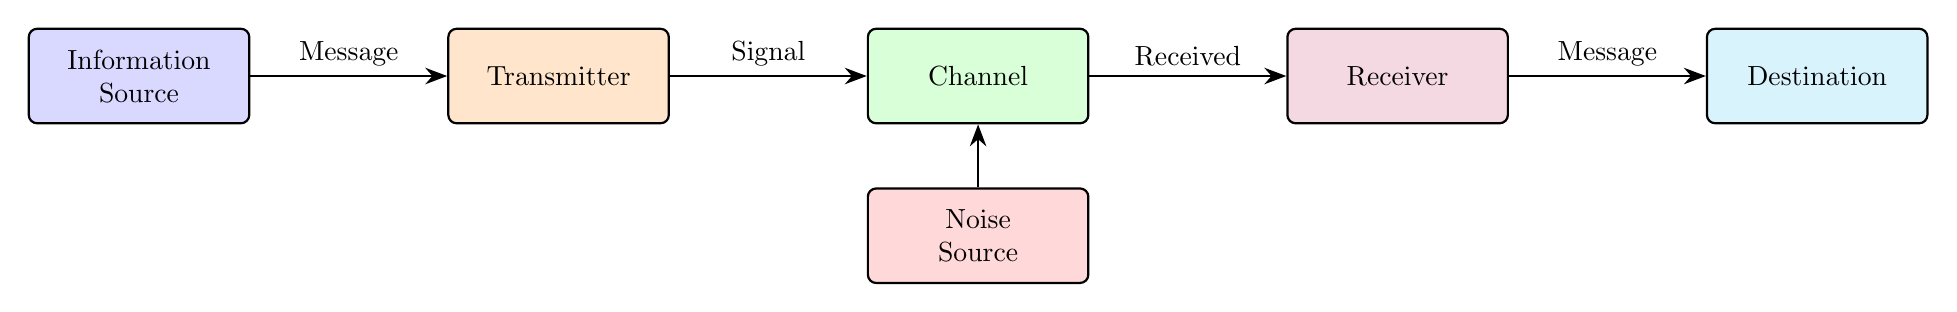
\begin{tikzpicture}[
    node distance=2.5cm,
    box/.style={rectangle, draw, thick, minimum width=2.8cm, minimum height=1.2cm, align=center, rounded corners=3pt},
    arrow/.style={-{Stealth[scale=1.2]}, thick}
]

\node[box, fill=blue!15] (src) {Information\\Source};
\node[box, fill=orange!20, right=of src] (tx) {Transmitter};
\node[box, fill=green!15, right=of tx] (ch) {Channel};
\node[box, fill=red!15, below=0.8cm of ch] (noise) {Noise\\Source};
\node[box, fill=purple!15, right=of ch] (rx) {Receiver};
\node[box, fill=cyan!15, right=of rx] (dst) {Destination};

\draw[arrow] (src) -- (tx) node[midway, above] {Message};
\draw[arrow] (tx) -- (ch) node[midway, above] {Signal};
\draw[arrow] (noise) -- (ch);
\draw[arrow] (ch) -- (rx) node[midway, above] {Received};
\draw[arrow] (rx) -- (dst) node[midway, above] {Message};

\end{tikzpicture}
\end{document}
